\documentclass[a4paper,10pt]{article}

\usepackage{enumitem}
\usepackage[utf8]{inputenc}
\usepackage{textcomp}
\usepackage{xspace}
\usepackage[italian,english]{babel}
\usepackage[pdftex]{graphicx}
\usepackage{fullpage}
\usepackage{amsmath}
\usepackage{caption}
\usepackage{subcaption}
\usepackage{multirow}
\usepackage{amsfonts}
\usepackage{booktabs}
\usepackage{wrapfig}
\usepackage[numbers]{natbib}

\usepackage{listings}
\lstset{
	basicstyle=\fontsize{8}{12}\ttfamily,
	inputencoding=utf8,
	language=Python,
	numbers=left,
	numberstyle=\tiny,
	tabsize=2,
	frame=single,
	backgroundcolor=\color{gray},
}

\setenumerate[2]{label=\alph*.}

\usepackage{color}
\definecolor{gray}{gray}{0.9}

\usepackage{hyperref}
\hypersetup{
	colorlinks=true
}
\usepackage{hypcap}

\include{commands}

\begin{document}

\thispagestyle{empty}
\begin{center}
	\leavevmode
	\large
	\begin{tabular}{ r l }
		\multirow{2}{*}{\includegraphics[width=2cm]{img/unipd_logo.png}} & \textsc{Università degli studi di Padova}\par \\
			& \textsc{Corso di laurea magistrale in Ingegneria Informatica} \\
	\end{tabular}
		
	\vfill
	{\Large Sistemi Intelligenti \par Relazione del progetto} \par
	\vskip .5cm
	\textbf{{\LARGE A spam classifier based on Bayesian networks}}\par
	\vskip 3cm
	\normalfont
	
	\begin{tabular}{ c c }
		\large Alberto \textsc{Franzin} & \large Fabio \textsc{Palese} \\
		\normalsize 1012883 & \normalsize 1033575 \\[1cm]
	\end{tabular}
	\normalfont
	\vskip 4cm
	
	\begin{flushright}
		\emph{Docenti:}\\
		Prof. Silvana \textsc{Badaloni}\\
		Prof. Francesco \textsc{Sambo}
	\end{flushright}

	
	\vfill
	{\large AA 2012-13}
\end{center}
\cleardoublepage

\pagenumbering{roman}

\begingroup
	\hypersetup{linkcolor=black}
	\setcounter{tocdepth}{3}
	\tableofcontents
\endgroup

\newpage

\pagenumbering{arabic}

\section{Introduction}
This project has been developed as part of the course in Intelligent Systems, a.y. 2012/13, by Alberto Franzin and Fabio Palese.

The project consists in a spam classifier for emails based on Bayesian networks, a probabilistic model to represent conditional dependencies between random variables that can be used as a classifier in the field of supervised learning.

The code and the documentation of the project is available at\\ \url{http://code.google.com/p/sist-int-2012project/}.

This documents is divided in four sections: in the first one, we briefly introduce the theory behind Bayesian networks, in the second section we describe the working of project, then we show the results that we have obtained and finally we draw the conclusions.

\section{Bayesian networks}
\subsection{The Bayes' theorem}
The theorem stated by Thomas Bayes says that, given two events $H$ (hypothesis) and $T$ (thesis), respectively with probabilities $P(H)$ and $P(T)$:
\[ P(H|T) = \frac{P(H \cap T)}{P(T)} = \frac{P(T|H)P(H)}{P(T)}, \]
that is: the probability that the hypothesis is verified, given that we know the thesis, comes from the probability of observing the thesis knowing the hypothesis occurred, times the ratio of the single probabilities of hypothesis over the thesis.

We call $P(H)$ the \textit{prior} probability of $H$, that is our initial, unconditioned knowledge about $H$, $P(T|H)$ is the \textit{likelihood}, i.e. the function of the parameter having a certain value given the outcome, and $P(H|T)$ the \textit{a posteriori probability of $H$ given $T$}, that describes our modified knowledge about event $H$ given that we know the event $T$ has occurred.

While the Bayes' theorem is universally accepted, there are two possible interpretations. The first one follows the frequentist approach, that relies on the knowledge (or the possibility of discovering) of the probability of an event, given the hypotheses. Frequentists (ideally) have an infinite amount of data. The other approach is the bayesian one, which tries to infer the hypotheses of an event, given the data. It's often said that under this view, the probability measures a subjective degree of belief on an event: the probability that we assign to an hypothesis reflects how much we do believe in that hypotheses.

For example, if we throw a coin one million times, we expect to see about 500 thousands heads. But if we see, say, only 200K heads, then we may suspect that the coin is biased.

A typical application of Bayes' theorem is diagnostic. Given the results of a medical exam and the accuracy of the exam (percentage of false positives and false negatives), we can estimate the probability of effectively having the disease.

\subsection{Bayesian networks}
A Bayesian network is a probabilistic model that defines a probability distribution over a graph of variables. The nodes represent the events, and the (directed) arcs mean the probabilistic relationship between events. An arc going from node $X$ to node $Y$ with an associated probability $p$ means that $Y$ is conditionally dependent from $X$ with probability $p$.

The name ``Bayesian network'' has been coined by Judea Pearl (see \cite{pearl1985bayesian}), to highlight three characteristics of this model:

\begin{enumerate}[noitemsep]
  \item the \textit{judgmental origin of the quantifiers};
  \item the \textit{ability of update beliefs};
  \item the \textit{structure of influence networks stem from the dominant role \textit{causality} plays in the formation of these networks}.
\end{enumerate}

More informations on Bayesian networks can be found in \cite{mitchell2005draft} and \cite{bayestheorytool}.

In figure \ref{fig:bayesnet} we see an example of a Bayesian network, describing the following situation: an alarm may be triggered by two events, a burglar entered into the house, or an earthquake. When the alarm rings, we may receive a call from John or Mary, who both can hear the alarm. The conditional dependence can be represented with the example probabilities in table \ref{tab:probsbn}.

\begin{wrapfigure}{l}{8cm}
  \begin{center}
    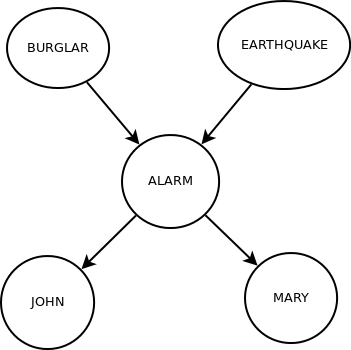
\includegraphics[width=0.4\textwidth]{img/bayes_network.png}
    \caption{An example of a Bayesian network.}
    \label{fig:bayesnet}
  \end{center}
\end{wrapfigure}

\begin{table}[h]%[!htb]
    \begin{minipage}{.25\linewidth}
      %\caption{A burglar entered the house.}
      \centering
        \begin{tabular}{cc}
          \toprule
          $B$ & $P(B)$ \\
          \midrule
          $+b$  & 0.001 \\
          $\neg b$  & 0.999\\
          \bottomrule
          \toprule
          $E$ & $P(E)$ \\
          \midrule
          $+e$  & 0.002 \\
          $\neg e$  & 0.998\\
          \bottomrule
        \end{tabular}
    \end{minipage}%
    \begin{minipage}{.4\linewidth}
      \centering
        %\caption{An earthquake occurred.}
        \begin{tabular}{cccc}
          \toprule
          $B$ & $E$ & $A$ & $P(A|B,E)$\\
          \midrule
          $+b$     & $+e$     & $+a$     & $0.95$ \\
          $+b$     & $+e$     & $\neg a$ & $0.05$ \\
          $+b$     & $\neg e$ & $+a$     & $0.94$ \\
          $+b$     & $\neg e$ & $\neg a$ & $0.96$ \\
          $\neg b$ & $+e$     & $+a$     & $0.29$ \\
          $\neg b$ & $+e$     & $\neg a$ & $0.71$ \\
          $\neg b$ & $\neg e$ & $+a$     & $0.001$ \\
          $\neg b$ & $\neg e$ & $\neg a$ & $0.999$ \\
          \bottomrule
        \end{tabular}
    \end{minipage}
    \begin{minipage}{.35\linewidth}
      %\caption{A burglar entered the house.}
      \centering
        \begin{tabular}{ccc}
          \toprule
          $A$ & $J$ & $P(J|A)$ \\
          \midrule
          $+a$     & $+j$     & $0.9$ \\
          $+a$     & $\neg j$ & $0.1$ \\
          $\neg a$ & $+j$     & $0.05$ \\
          $\neg a$ & $\neg j$ & $0.95$ \\
          \bottomrule
          \toprule
          $A$ & $M$ & $P(M|A)$ \\
          \midrule
          $+a$     & $+m$     & $0.7$ \\
          $+a$     & $\neg m$ & $0.3$ \\
          $\neg a$ & $+m$     & $0.01$ \\
          $\neg a$ & $\neg m$ & $0.99$ \\
          \bottomrule
        \end{tabular}
    \end{minipage}%
    \caption{Probabilities of the Bayesian network in figure \ref{fig:bayesnet}.}
    \label{tab:probsbn}
\end{table}

$P(B)$ and $P(E)$ are, respectively, the probability of a burglar having entered the house, and the probability of having detected an earthquake; $P(A|B,E)$ is the probability that the alarm rings, given we know the status of $B$ and $E$; $P(J|A)$ and $P(M|A)$ are the probabilities that we receive a call from John and Mary, given the status of the alarm. The only ``stand-alone'' probabilities that we can define are the ones of the \textit{evidence} variables (we do know them), namely the burglar and the earthquake. All the other events can only have a probability conditioned to the occurrence of its direct ancestors. To know the probability of one of these events alone, we have to compute the total probability of the event.
With the numbers given in the example, if Mary hasn't called, then the alarm was off w.p. $0.99$. Knowing this, the probability that there has been a burglary is roughly $1.12 \times 10^{-6}$.

We can also read the diagram backward, from bottom to top: for example, $A$ depends on both $J$ and $M$: if the alarm occurs, then it is likely that John or Mary have called.

\subsubsection{Conditional independence}
Given three events $A$, $B$ and $C$, we say that $A$ and $B$ are \textit{conditionally independent} if $P(A \cap B | C) = P(A|C)P(B|C)$, or, equivalently, $P(A | B \cap C) = P(A|B)$. In a bayesian network, two variables (events) are independent if they are not linked by just unknown variables. For example, if we do not know anything about the alarm, then burglary and earthquake are independent, since we cannot infer anything about them.

If the alarm rings, and we know that an earthquake has occurred, then it becomes less likely that a burglar has entered the house, since we already have a cause that can have triggered the alarm. This is the \textit{explaining away} effect.

When an event has multiple causes, then we say that seeing one cause of the possible ones may ``explain away'' all the other causes, because it becomes less likely for them to happen.

\subsection{The \textit{naive} approach}
Bayesian networks require a huge number of variables: because of the chain rule of probabilities, if a node has $k$ incoming arcs, then we need $2^k$ variables. Furthermore, it may difficult to compute the joint probability of variables.

The \textit{naive} approach works under the assumption of independence among variables. It is called ``naive'' since this assumption is very string but not always realistic. Consider now the case of a spam mail: if we read the words ``buy replica watches'' (which already is a set of words) we expect to read some watch brands too. Anyway, while considering all the subset of words requires exponential time, the assumption of independence allows us to consider each word alone, pulling it out of context, and therefore it allows the computation to drop from exponential to linear time. Moreover, the calculation of the probabilities is now reduced to a product of the single probabilities of the variables. Maybe surprisingly, this approach works quite well in practice, being both fast and accurate, despite its ``naivety''.

\subsection{Naive Bayes for spam classification}
We describe now how to apply the theory above to a real problem, in this case the classification of a mail as a spam mail or a valid mail.

We define a mail as \textit{spam} if it contains undesidered or illegal content. A valid mail is conversely defined as \textit{ham}.

The naive approach that tells us to consider each words alone, allows to represent the document as a \textit{bag of words}, which is a dictionary containing the words encountered in the mails, each one associated with its frequency (see figure \ref{fig:nbs}). We read the diagram this way: if we have a mail, what is the probability of reading the word \verb!word1!, knowing the mail is spam? And \verb!word2!? And so on.

\begin{figure}[h]
  \begin{center}
    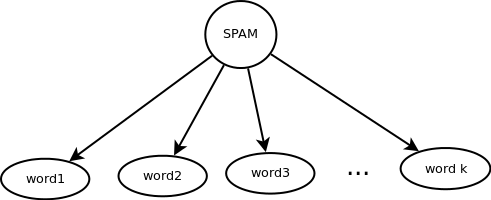
\includegraphics[width=0.6\textwidth]{img/bayes_network_spam.png}
    \caption{Naive Bayes network for spam classification: \textit{bag of words} representation.}
    \label{fig:nbs}
  \end{center}
\end{figure}

In addiction to the words, often we can easily distinguish a spam email from a valid one by looking at it and recognizing some of these characteristics: bad grammar, bad syntax, undue use of images, lots of links, and many others. Detecting these features may be useful to correctly classify an email.

\subsubsection{Algorithm}
\paragraph{Data structures}
To represent the \textit{bag of words}, we need a dictionary of \verb!(word, stats)!. We need also to store the statistics for the various features detected, in an analogous data structure containing \verb!(feature, stats)!. In both cases, the statistics have to distinguish between frequency in spam mails and frequency in ham mails. This is enough to contain all the informations we need to know about the training set.

The statistics of the mails in the validation set and in the test set will be stored in similar data structures, but their stats will contain only the number of times the words and the featured have been observed, since the network does not know the status of the mail when these operations are performed.

\paragraph{Training}
To train the system, we have to feed the network with the training set. The network will read the mails, extract the actual content and adjust the count of both words and features.

\paragraph{Validation}
The next step is to measure how good the results of the training are. To accomplish this, we provide the network other mails of which we already know the status, to later check the results. The network will read each mail, extract the stats and compare them to the overall statistics generated during the training step. The result of the classification will be the class that maximizes the probability for the mail to belong to that class.

\paragraph{Testing}
Now we compute the final accuracy of the bayesian network, in the same way as the validation, on a larger set of mails.

For both validation and testing, the bayesian network can track its previous work and update the probabilities, so to keep its tables up-to-date and to reflect the actual nature of the dataset.

\subsubsection{Computing the probability}
\label{computeprob}
From the previous sections, we know that for each word $$P_{spam|word} = \frac{P_{word|spam}P_{spam}}{P_{word}}, \quad P_{ham|word} = \frac{P_{word|ham}P_{ham}}{P_{word}}.$$ Since $P_{word}$ is just a normalizer and is the same for both the terms, it can be omitted. Then, when we analyze the training set, we read the words knowing the status of the mail they belong to, and thus at the end of the training step we can say that $$P_{word|spam} = \frac{\mbox{\# occurrences of word in spam mails}}{\mbox{\# total occurrences of word}}, \quad P_{word|ham} = \frac{\mbox{\# occurrences of word in ham mails}}{\mbox{\# total occurrences of word}}.$$

We need to compute these probabilities for each word we encounter when reading a mail. Finally we compute the total probability for the mail of being spam and ham, which, for the naive assumption of independence, will be respectively $$P_{spam} = \prod_{words \in mail} P_{spam|word} \quad\mbox{and}\quad P_{ham} = \prod_{words \in mail} P_{ham|word}.$$ The outcome of the classification will be the class that maximizes these two probabilities.

\subsubsection{Updating the knowledge}
When the Bayesian network classifies a mail, it uses the result to update its knowledge. This can be done by just updating the counter of the statistics of the dictionary associated with the network.

\section{Implementation}
Here we describe our implementation of a Naive Bayes spam classifier. Further documentation is available with the package.

The project has been written in Python. It requires two external modules, \verb!bs4! (\verb!BeautifulSoup!) to parse a text and \verb!Ply! to perform the lexical analysis of a text.

\subsection{Structure}
The package is composed as follows:
\begin{description}[noitemsep]
  \item[spam\_bayes] the module contianing the \verb!__main__! class;
  \item[naive\_bayes] the module defining the Bayesian network;
  \item[config] contains some general configurations, manages the settings defined by the user;
  \item[trainer] contains the trainer;
  \item[classifier] applies the Bayesian logic to classify a mail;
  \item[lexer] implementing the lexical analyzer to compute the statistics;
  \item[utils] with some methods used in more classes.
  \item[gen\_stat] defines the objects to describe the statistics for words and features of the global network;
  \item[test\_stat] defines the objects to describe the statistics for words and features of a single mail of unknown status.
\end{description}

Image \ref{fig:uml} shows the interconnection between the classes.
\begin{figure}[h]
  \begin{center}
    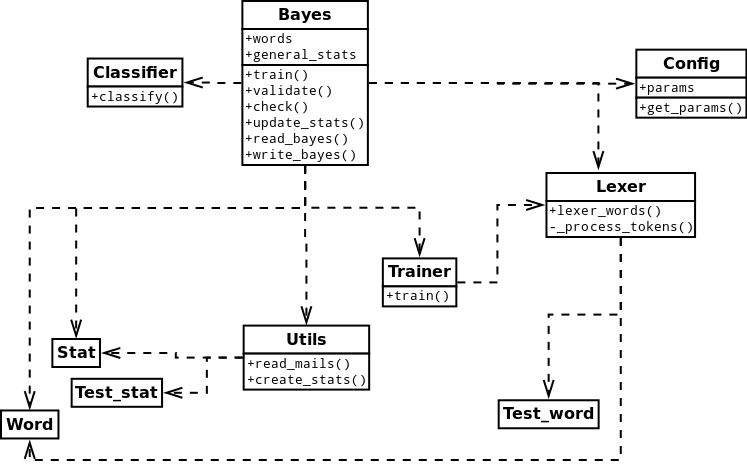
\includegraphics[width=0.6\textwidth]{img/uml.png}
    \caption{UML diagram of the classes.}
    \label{fig:uml}
  \end{center}
\end{figure}

The file \verb!spam_bayes.conf! allows the user to configure the parameters.

\subsubsection{Notes on implementation}
\label{notesonimpl} In section \ref{computeprob} we have discussed how to compute the probability of being spam and ham, and we have discarded the total probability of each word, since it's only a normalizer, equal for both the terms. We can further simplify the calculation, assuming to not know the a priori probability for a mail to be spam or ham, and so considering it $0.5$. This is true when the classification begins, and the bag of words is still empty, or when the number of spam and ham mails are almost equal. However, this works also when there is a disproportion between the numbers of spam and ham mails. Thus, being this probability equal for both terms, it can be discarded.

We need also to be careful when computing the total probability, since if the probability of being spam or ham associated to a word is $0$ (e.g. no spam/ham mails contain the word), the total probability will be $0$ regardless of all the other probabilities. To avoid this, we add a smoothing value to both the numerator and denominator in $P_{spam|word}$ and $P_{ham|word}$. Thus, the formula for spam becomes $$P_{word|spam} = \frac{\mbox{\# occurrences of word in spam mails} + k}{\mbox{\# total occurrences of the word} + |C|\times k},$$ where $|C|$ is the number of possible classes, in our case 2, spam and ham, and $k > 0$ is the smooth value. If $k=1$ it is called Laplace smoothing.

Furthermore, other calculation can be avoided. Words like articles or conjunctions are very common in every meaningful text, so we expect them to appear many times in both spam and ham mails. We can extend this observation, considering that every word which has a probability of being spam close to $0.5$ will also have a very similar probability of being ham, since their sum has to be $1$. Thus, also these words bring very little contribution to the spamminess of a mail, and can therefore be ignored. We provide a customizable threshold to allow the user to set the preferred deviation from the half, for the word to be counted into the probability. Also, only words that have been already found some times will be taken into account, since too few occurrences of the word may not be statistically relevant.

We have discussed so far about what to do when we read a word which has already been met before. In the case that the classifier encounters a word for the first time, we have seen that the best action is to do nothing: the status of the mail will be guessed by using the other words and features, the word just gets inserted into the bag of words, according to the status computed, so that it can be used in the following rounds.

\section{Tests and results}
\subsection{Dataset}
The dataset used is the SpamAssassin Public Corpus provided by SpamAssassin at \url{http://spamassassin.apache.org/publiccorpus/}, freely available for development purposes (maintainers warn to not use the dataset for training a live system). It contains about 6400 mails in english language, collected from 2002 to 2005, with approximately the 31\% of the mails being spam.

\subsection{Modalities}

\subsection{Features of spam and ham mails}
\label{featuresused} The following features have been selected as relevant and are tracked by the network:
\begin{itemize}[noitemsep]
  \item the number of words written in uppercase characters: since it is considered the equivalent of screaming, many spammers use this gross trick to gain attention;
  \item the number of urls found: we expect to find a lot of addresses of websites where to buy goods or where some criminal activity will be performed (phishing, stealing credentials, etc.);
  \item the number of email addresses: for the same reason of the previous feature. Furthermore, spammers operate on a large scale, so it is possible for a spam mail to have multiple recipients;
  \item the number of words shorter than a given threshold (given as a parameter): a trick to fool a system based on word classification is to hide the words. One of the most common and easier way of accomplish this, is to separate each letter with spaces. Since our token separation relies on whitespaces between words, a word like \texttt{s\textvisiblespace p\textvisiblespace a\textvisiblespace m} (with spaces between characters), which a human will easily understand as a single one, will be classified by the network as four different words. In a common, correct plain english text, the ratio of short words like \verb!a! or \verb!I! will be substantially lower, not to mention other random letters;
  \item the number of non-address words longer than a given threshold (parameter): similarly to the previous feature, a spam mail is likely to contain a number of very long, meaningless words much higher than a ham mail. Since there aren't many very long legit words\footnote{The average length of english words is slightly higher than 5 (\url{http://www.puchu.net/doc/Average_Word_Length}), while the majority of words appearing in a text is from 2 to 5 letters long. \citep{STUL:STUL109}}, this is a reasonable feature to track;
  \item the number of words in the form \verb!username@host!: the tests have shown that the ham mails in the SpamAssassin Public Corpus contain many tokens of this type;
  \item the number of words in ``title'' format (first letter capital, remaining letter lowercase);
  \item the number of words in a mail.
\end{itemize}

Many other interesting features can also be used: for example, a heavy use of images as text replacement, the consistency of the email header, the consistency of the urls with the link they claim to go, the list of people the user have mailed before, the provenance of the mail from a known spammer or IP range, the correctness of words (by checking a dictionary), to name a few. All of these features require a semantic analysis of the mail, which goes beyond the purpose of this project, since no one of these features is directly connected to Bayesian networks. Nonetheless, all of these features can be used by a Bayesian network, just like the previous ones, and are very likely to increase the accuracy of the classification.

It should be noted that while some of these features are common for the majority of spam, some others are derived from our particular mail archive. Moreover, since many of the mails in the archive are ten years old, more recent spam mails may contain different features.% The maintainers of the archive warn to use the archive only for development purposes, not in a live system.

\subsection{The design parameters}
The Bayesian network requires some parameters to be tuned: for example, the ``spamicity'' threshold (how much the normalized probability of being spam should be to be really considered as spam), or the ``weight'' of the feature stats with respect to the word stats when computing the final probability. Different parameter configurations lead to obtain different accuracy values, so we have to choose the best one.

We'll now present the results obtained. Since there are multiple degrees of freedom, we show how the accuracy varies when trying to change one single parameter at time, all the other ones being set to their optimal value. Because of the random choice of the emails used for training, validation and testing, multiple tests have been performed, and the results in the following paragraphs are the medians of the values observed.

\paragraph{Size of the training and validation sets}
For finding the best size of the training set, we have begun with few mails, then we have tried to increase the size of the training set until the accuracy has started to decrease (the \textit{early stopping} technique). The size of the validation set is a quarter of the size of the training set. Each value in table \ref{tab:sizebags} is intended to be doubled, being the number of mails for each class to be used.

\begin{center}
\begin{table}[h]
\begin{minipage}{.5\linewidth}
\begin{tabular}{cccc}
\toprule
\multicolumn{2}{c}{Size of sets} \\
\cmidrule(r){1-2}
Training & Validation & \shortstack{Validation\\ accuracy} & \shortstack{Testing\\ accuracy}\\
\midrule
50   & 12     & 0.5416667 & 0.739\\
100  & 25     & 0.78 & 0.7725 \\
200  & 50     & 0.72 & 0.7935 \\
500  & 125    & 0.788 & 0.842 \\
800  & 200    & 0.71 & 0.8515 \\
1000 & 250    & 0.73 & 0.849 \\
\bottomrule
\end{tabular}
\end{minipage}
\begin{minipage}{.5\linewidth}
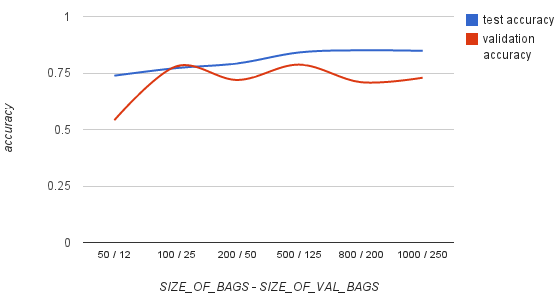
\includegraphics[width=1\textwidth]{img/tests/size_bags.png}
    \label{fig:sizebags}
\end{minipage}
\caption{Accuracy with varying size for training set and validation set.}
\label{tab:sizebags}
\end{table}
\end{center}

As we see, the best accuracy is obtained using 800 spam mails and 800 ham mails for training, and 200+200 mails for validation. Furthermore, if we compare all the results, we observe that with fewer mails the variance of the results is higher.

\paragraph{Size of test sets}
As for training and validation set, we look for the optimal size of the training set. Because of the self-improving nature of Naive Bayes networks, we expect the accuracy to grow along with the size of the training set. Results of the trials are shown in table \ref{tab:sizetest}.

\begin{center}
\begin{table}[h]
\begin{minipage}{.5\linewidth}
\begin{tabular}{cccc}
\toprule
Size of test set & \shortstack{Validation\\ accuracy} & \shortstack{Testing\\ accuracy}\\
\midrule
100  & 0.7575 & 0.82     \\
200  & 0.74   & 0.835    \\
500  & 0.7275 & 0.827    \\
800  & 0.6975 & 0.842605 \\
1000 & 0.71   & 0.8515   \\
\bottomrule
\end{tabular}
\end{minipage}
\begin{minipage}{.5\linewidth}
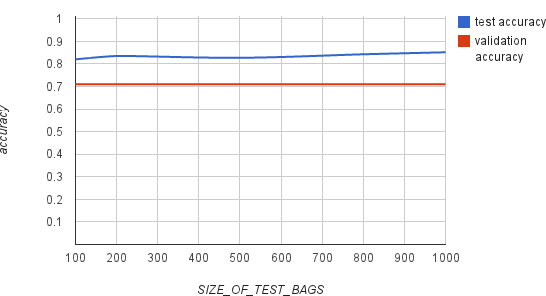
\includegraphics[width=1\textwidth]{img/tests/size_test.png}
    \label{fig:sizetest}
\end{minipage}
\caption{Accuracy with varying size of test sets.}
\end{table}
\label{tab:sizetest}
\end{center}

As expected, the more mails are processed, the higher accuracy we get. We stopped at 1000+1000 mails, because it takes a long time to process all the mails, and because the increment of accuracy begins to slow down.

\paragraph{``Spamicity'' threshold}
\label{spamthrtest} Another very important parameter is what is sometimes called the ``spamicity'' threshold, namely the value that the normalized probability $\frac{p_{spam}}{p_{spam} + p_{ham}}$ must reach for the mail to be classified as spam. This is crucial: a low threshold will bring in many false positives (good mails will be marked as spam), while a too high threshold will classify some spam mails as ham, thus having a lot of false negatives. Anyway, the choice of the threshold to be $0.5$ may not be obvious, since we may want to be more tolerant with words we have never met before, or we may consider the chance of false positive too bad for us, and therefore lift the threshold to ensure this fact, allowing at the same time some spam to pass through the filter. More importantly, we desire a similar number for false positives and false negatives, since this is an index of well-balanced classification. For this reason, this value is only the starting value of the threshold, which will be tuned by the classifier according to the number of misclassified items. Furthermore, given the nature of bayesian networks, a fair threshold guarantees that the classifier remains stable, meaning that it will continue guessing with the same ham and spam ratio, while a very unbalanced number of misclassifications will make the classifier leaning towards too many guesses of a single kind (the more mails are misclassified as spam, the more words will erroneously contribute to spam in future classifications, same for ham).

\begin{center}
\begin{table}[h]
\begin{minipage}{.5\linewidth}
\begin{tabular}{cccc}
\toprule
Threshold & \shortstack{Validation\\ accuracy} & \shortstack{Testing\\ accuracy}\\
\midrule
0.1  & 0.725 & 0.834\\
0.2  & 0.71 & 0.8515 \\
0.3  & 0.77 & 0.8305 \\
0.4  & 0.7 & 0.8595 \\
0.5  & 0.72 & 0.8455 \\
0.6  & 0.7125 & 0.841 \\
0.7  & 0.74 & 0.839 \\
0.8  & 0.7 & 0.848 \\
0.9  & 0.705 & 0.8305 \\
\bottomrule
\end{tabular}
\end{minipage}
\begin{minipage}{.5\linewidth}
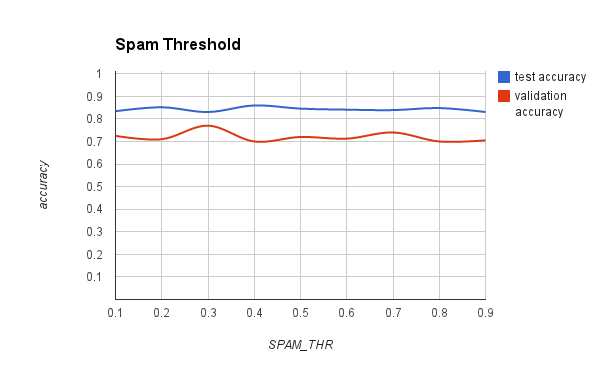
\includegraphics[width=1\textwidth]{img/tests/spam_thr.png}
    \label{fig:spamthr}
\end{minipage}
\caption{Accuracy with varying ``spamicity'' threshold.}
\end{table}
\label{tab:spamthr}
\end{center}

We see that the accuracy is similar for all the starting values. Anyway, when looking at the final value that the threshold take, we see that most of the times it lies around 0.2, so this is our default value. The other starting values get a similar accuracy because when having multiple errors in the beginning, the threshold changes rather quickly.

\paragraph{Relevance threshold}
As we have already discussed in section \ref{notesonimpl}, we provide a customizable threshold to exclude from computation the words and the features that give little contribution to the final probabilities. In table \ref{tab:relevance} we see what is the most convenient value.

\begin{center}
\begin{table}[h]
\begin{minipage}{.5\linewidth}
\begin{tabular}{ccc}
\toprule
Threshold & \shortstack{Validation\\ accuracy} & \shortstack{Testing\\ accuracy}\\
\midrule
0.15  & 0.6925 & 0.703  \\
0.2   & 0.6925 & 0.8025 \\
0.25  & 0.71 & 0.8515   \\
0.3   & 0.605 & 0.798   \\
0.35  & 0.71 & 0.6665   \\
\bottomrule
\end{tabular}
\end{minipage}
\begin{minipage}{.5\linewidth}
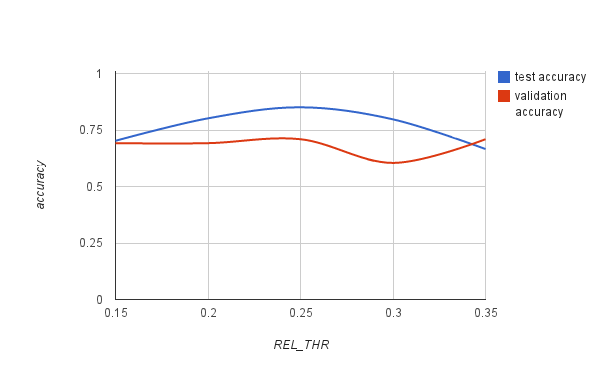
\includegraphics[width=1\textwidth]{img/tests/rel_threshold.png}
    \label{fig:relthreshold}
\end{minipage}
\caption{Accuracies obtained when varying the relevance threshold.}
\end{table}
\label{tab:relevance}
\end{center}

\paragraph{Feature/words stats proportion}
Another problem is to determine how much weight should we assign to the features statistics, and how much to the word statistics.

The final formula for spam is $p_{spam} = W \times p_{fs} + (1-W) \times p_{ws}$, where $p_{spam}$ is the probability of the mail being spam (yet to be normalized), $p_{fs}$ is the probability of being spam computed using the statistics of the features, $p_{ws}$ is the probability of being spam computed using the statistics of the words, and $W$ is the parameter we want to adjust. The formula for ham is the dual.

A value close to $1$ will lead to a classification based solely on the features, thus almost ignoring the actual content of the mail. A low value will instead disregard the features, and therefore many useful and common characteristics of spam mails.

\begin{center}
\begin{table}[h]%[!htb]
\begin{minipage}{.5\linewidth}
%\begin{scriptsize}
\begin{center}
\begin{tabular}{ccccc}
\toprule
Threshold & \shortstack{Validation\\ accuracy} & \shortstack{Testing\\ accuracy} \\
\midrule
0.0001 & 0.7025 & 0.8595 \\
0.001  & 0.7125 & 0.8275 \\
0.01   & 0.6925 & 0.832  \\
0.1    & 0.6725 & 0.801  \\
0.2    & 0.745  & 0.7945 \\
0.4    & 0.7325 & 0.7795 \\
0.6    & 0.6925 & 0.739  \\
0.8    & 0.73   & 0.7115 \\
\bottomrule
\end{tabular}
\end{center}
%\end{scriptsize}
\end{minipage}
\begin{minipage}{.5\linewidth}
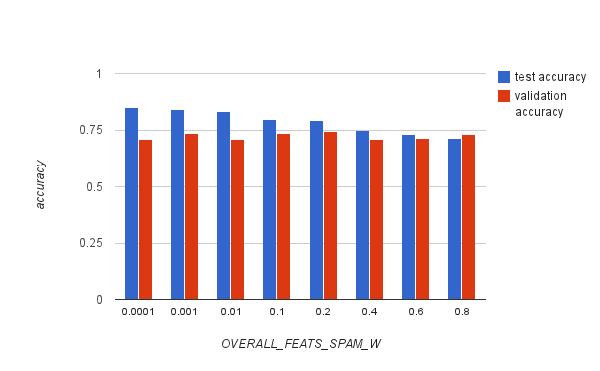
\includegraphics[width=1\textwidth]{img/tests/feats_threshold_1.png}
    \label{fig:featuresthreshold}
\end{minipage}
\caption{Validation and final accuracies, with varying feature statistics thresholds.}
\label{tab:featsthr}
\end{table}
\end{center}

We clearly see (table \ref{tab:featsthr}) that the more the threshold approaches zero, the better results it yields. This means that, at least with the dataset we are using, a classifier based only on words works better than a classifier which accounts also the general features of the mail. It is interesting to note that the validation accuracy remains almost at the same level, while the real difference comes out during the testing step, when a much higher number of mails are processed, and the network can thus learn much more. 

\subsection{Analysis of results}
Here we show and analyze some interesting results observed. Of course, these statistics apply only for the SpamAssassin dataset, and may not be generalized.
% \begin{center}
% \begin{tabular}{lcc}
% \toprule
% & \multicolumn{2}{c}{Occurrences} \\
% \cmidrule(r){2-3}
% Feature & \# in spam & \# in ham \\
% \midrule
% \# of all-caps words                            & 10    & 0.1 \\
% \# of alphanumerical words                      & 20    & 0.2 \\
% \# of string in user/hosts form                 & 50    & 0.3 \\
% \# of links                                     & 100   & 0.4 \\
% \# of mail addresses                            & 10    & 0.1 \\
% \# of all lowercase words                       & 20    & 0.2 \\
% \# of words with only the first letter capital  & 50    & 0.3 \\
% \# of ``short words''                           & 10    & 0.0 \\
% \# of non-address ``very long'' words           & 100   & 0.4 \\
% \# of non-valid words                           & 50    & 0.3 \\
% \# of numbers                                   & 100   & 0.4 \\
% \bottomrule
% \end{tabular}
% \end{center}

As expected, ``very short'' and ``very long'' words (out of our thresholds) are mostly common in spam mails, as well as all-caps words, non-valid words and mail addresses. Spam mails also contain an average number of words higher than ham ones. Surprisingly, in the SpamAssassin dataset ham mails contain more links than spam mails.

%\paragraph{Most common words}
It's interesting also to look at the statistics of the single words. We have already discussed about how the distribution of unusually long words. In our dataset, the words that contribute most to ham are technology-related words like debian, cpp, gaim, 0xdeadbeef (hex code used by \textsc{IBM}). Spam mails, instead, are characterized by meaningless words and words that suggest the selling of some good, in particular drugs, as for example botanical, dieting, aphrodisia.

% \begin{center}
% \begin{tabular}{cc}
% \toprule
% Words in spam & Words in ham \\
% \midrule
% \# of all-caps words                            & matthias \\
% \# of alphanumerical words                      & 0xdeadbeef \\
% \# of string in user/hosts form                 & gaim \\
% \# of links                                     &  \\
% \# of mail addresses                            & 10 \\
% \# of all lowercase words                       & 20 \\
% \# of words with only the first letter capital  & 50 \\
% \# of ``short words''                           & 10 \\
% \# of non-address ``very long'' words           & 10 \\
% \# of non-valid words                           & 50 \\
% \# of numbers                                   & 10 \\
% \bottomrule
% \end{tabular}
% \label{tab:commonwords}
% \end{center}

\section{Conclusions}
We have seen that the Nave Bayes approach works quite well when classifying a dataset, despite its simplicity. The training requires some hundred of mails, but after this the performance gets better thanks to the bayesian logis, that updates the probability according to its own previous work. Thus, the more mails are processed, the higher accuracy we get (if we start from an adequate accuracy: if we start from a low quality classifier, our results would remain very bad).

Since the network has to be trained on a specific dataset, clearly the results reflect the composition of the mail corpus used. Using the SpamAssassin dataset, we have found that ham mails are likely to contain more links than spam ones; we would have expected the opposite. As expected, the most common words are useless single characters, and common english words like articles, conjunctions, etc. that do not bring any contribution to the mail spamminess.

We have also seen that, with this implementation and this dataset, computing the features brings very little contribution to the status of a mail, and a word-based classification is more precise.

Note that a more complex system, better if integrated into a mail server or client, can surely achieve higher accuracy. We have already named a few features that can be added to the classifier to improve its performance. Anyway, we have shown that a very simple and ``naive'' Bayesian classifier can work pretty well with little data and a handful of key features.

The code can also be surely optimized, with a better knowledge of Python and with some code restructuration.


% %aggiunge la bibliografia all'indice
 %%niente sezioni anche qui, ovvio....
%\clearpage

\bibliographystyle{plainnat}
\bibliography{biblio}
\addcontentsline{toc}{section}{References}

\end{document}
